\section{Entwicklungsprozess}
Es wurden verschiedene Technologien zur 3D-Darstellung verglichen, darunter OpenGL, WebGL, Babylon und Three.js.
Nach der Erstellung von Prototypen mit Three.js und Pythreejs fiel die Entscheidung, NumPy für die mathematischen Berechnungen zu verwenden.
Daraufhin wurde eine Animationslogik entwickelt, um die Bewegungen im Projekt darzustellen. Schließlich wurde die Klasse Environment entworfen,
um den Code wiederverwendbar und verständlicher zu gestalten.

\subsection{Wahl der Rendering-API}
Zu Beginn des Entwicklungsprozesses wurden verschiedene Technologien zur Darstellung und Manipulation von 3D-Grafiken miteinander verglichen.
Dabei standen OpenGL, WebGL, Babylon und Three.js im Fokus.
Jede dieser Technologien bringt spezifische Vor- und Nachteile mit sich, die im Hinblick auf die Anforderungen des Projekts abgewogen wurden.
Anschließend wurde ein Prototyp auf Basis von Three.js erstellt und einer auf Basis von Pythreejs um die Eignung dieser Tools 
für das Projekt zu validieren. 


\subsubsection{OpenGL}
OpenGL überzeugte durch seine Plattformunabhängigkeit, da es auf verschiedenen Betriebssystemen wie Windows, macOS und Linux eingesetzt werden kann.
Dies ermöglicht Entwickler:innen, grafisch anspruchsvolle Anwendungen zu erstellen, die auf unterschiedlichen Systemen laufen, ohne dass spezifische Anpassungen nötig sind.
Es war besonders beliebt in Bereichen wie der 3D-Grafik, CAD-Software und der Spieleentwicklung.
Jedoch bringt OpenGL auch einige Einschränkungen mit sich.
Eine davon ist, dass OpenGL lokal auf dem Gerät installiert werden muss,
was zusätzliche Anforderungen an die Systemkonfiguration stellt und potenziell zu Kompatibilitätsproblemen führen kann.
Zudem benötigt es ein eigenes Anwendungsfenster, was die Integration in Web\-an\-wen\-dung\-en erheblich erschwert,
da moderne Web\-an\-wen\-dung\-en typischerweise ohne lokale Installation auskommen wollen \doublecite{opengl_doc}.

\subsubsection{WebGL}
WebGL stellt eine moderne, browserbasierte Alternative zu OpenGL dar, die auf denselben grundlegenden Prinzipien von OpenGL basiert.
WebGL läuft direkt in aktuellen Webbrowsern, ohne dass zusätzliche Software installiert werden muss, was einen entscheidenden Vorteil hinsichtlich der Zugänglichkeit bietet.
Durch die Nutzung von WebGL können Entwickler:innen 3D-Inhalte in Webseiten einbinden, was besonders für interaktive Webanwendungen von Bedeutung ist.
WebGL bietet ebenfalls eine plattformunabhängige Lösung, da es in allen gängigen Webbrowsern läuft, die HTML5 unterstützen. Allerdings ist WebGL relativ generisch und abstrakt aufgebaut.
Dies bedeutet, dass viele der für eine vollständige 3D-Anwendung notwendigen Funktionen manuell implementiert werden müssen, was den Entwicklungsaufwand
erheblich steigern kann. Zudem erfordert WebGL die Darstellung in einem separaten Browser-Tab,
was die Integration von 3D-Grafiken in eine bestehende Webanwendung erschwert \doublecite{webgl_wiki}.

\subsubsection{Babylon.js}
Babylon.js ist eine leistungsstarke 3D-Engine, die auf WebGL aufbaut und eine höher abstrahierte, fertige Lösung für die Entwicklung von 3D-Anwendungen bietet.
Babylon.js ermöglicht die schnelle Erstellung komplexer 3D-Szenen, ohne dass tiefgehende Kenntnisse über das zugrunde liegende Rendering-System notwendig sind.
Dies macht Babylon zu einer guten Wahl für Entwickler, die schnell funktionale 3D-Anwendungen erstellen möchten.
Jedoch kann diese umfangreiche Funktionalität auch nachteilig sein, insbesondere wenn nur bestimmte Teilaspekte einer 3D-Anwendung benötigt werden.
Babylon enthält beispielsweise ein vollständiges Physiksystem sowie ein Soundsystem, die für dieses Projekt nicht erforderlich sind und unnötige Komplexität hinzufügen.
Ein weiterer Nachteil von Babylon.js ist, dass es auch einen eigenen Browser-Tab benötigt,
um die Anwendung darzustellen,
was die Benutzererfahrung und Integration in Webanwendungen einschränkt \doublecite{BabylonJS, BabylonJS_specification, BabylonJS_Documentation_Physics}.

\subsubsection{Three.js}
Three.js, ebenfalls auf WebGL basierend, bietet eine abstrahierte Schnittstelle zur Erstellung von 3D-Inhalten,
geht dabei jedoch nicht so weit wie Babylon und bietet daher eine größere Flexibilität und Kontrolle.
Three.js liegt etwas näher an der Low-Level-Programmierung und ermöglicht es Entwickler:innen, die Details des Renderings anzupassen und zu optimieren.
Dies macht Three.js zu einem guten Kompromiss zwischen einfacher Nutzung und individueller Erweiterbarkeit,
da es eine gute Balance zwischen abstrahierter Funktionalität und den Möglichkeiten zur Anpassung von 3D-Szenen bietet.
Besonders für ein Projekt wie dieses, das im Rahmen einer Bachelorarbeit erweitert wird, erscheint diese Flexibilität von Vorteil,
da noch nicht klar ist, welche spezifischen Features in die Anwendung aufgenommen werden sollen. Im Gegensatz zu Babylon ist Three.js
leichtgewichtig und erlaubt eine genauere Anpassung an die Projektanforderungen.
Im Vergleich zu OpenGL oder WebGL, die eine Herangehensweise mit niedrigem Abstraktionsniveau bieten, überzeugt Three.js durch ein höheres Abstraktionsniveau,
was die Entwicklung beschleunigt und vereinfacht.
Wie bei den anderen Lösungen erfolgt die Darstellung auch in einem eigenen Browser-Tab, was eine ähnliche Einschränkung wie bei WebGL und Babylon darstellt.
Dennoch bietet Three.js aufgrund seiner Flexibilität und einfacheren Handhabung die beste Grundlage für dieses Projekt \doublecite{threeJS_manual}.

\subsection{Three.js-Prototyp}
Auf Basis dieser Überlegungen wurde im weiteren Verlauf des Entwicklungsprozesses ein einfacher Prototyp mithilfe der JavaScript-Bibliothek Three.js erstellt,
um zu überprüfen, ob die grundlegenden Funktionalitäten, die zur Erfüllung der Projektanforderungen notwendig sind, in Three.js enthalten sind.
Zu diesem Zweck wurde über den Node Package Manager (npm) das Paket live-server installiert, das es ermöglicht, eine HTML-Seite lokal zu hosten.
Auf dieser Seite wurde der Prototyp eingebunden und interaktiv getestet.
Abbildung \ref{fig:Verteilungsdiagramm-Prototyp} zeigt die Softwareumgebung und Einbettung des Prototyps in Form eines Verteilungsdiagramms.
\vspace{1em}

    \begin{figure}[H]
        \centering
        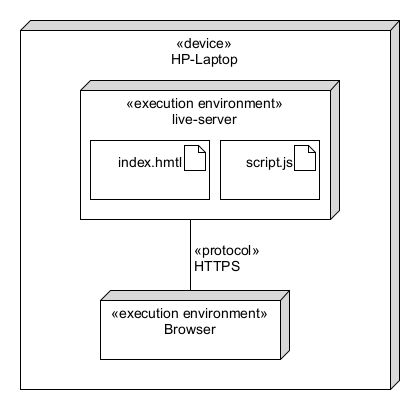
\includegraphics[width=0.8\textwidth]{images/diagramme/prototypKomponentendiagramm.png}
        \caption{Verteilungsdiagramm des Prototyps}
        \label{fig:Verteilungsdiagramm-Prototyp}
    \end{figure}

\vspace{1em}


Wie in der Abbildung zu sehen ist, kann auf den Prototyp über den Browser zugegriffen werden, was die Portabilität sicherstellt und dafür sorgt, dass 
auf einem potenziellen Endgerät keine zusätzliche Software installiert werden muss. Das Artefakt index.html ist die HTML-Seite, die zur inhaltlichen Darstellung
des Prototypen in einem eigenen Browsertab notwendig ist.
Inhaltlich umfasst Der Prototyp zunächst eine virtuelle Kamera, eine ambiente Lichtquelle sowie einen Würfel, die alle zu einer Szene hinzugefügt werden.
Für diese Schritte ist das Artefakt script.js zuständig, welches von index.HTML eingebunden wird.
Abbildung \ref{fig:Prototyp1} zeigt den Prototypen während der Ausführung im Browserfenster.

\vspace{1em}

    \begin{figure}[H]
        \centering
        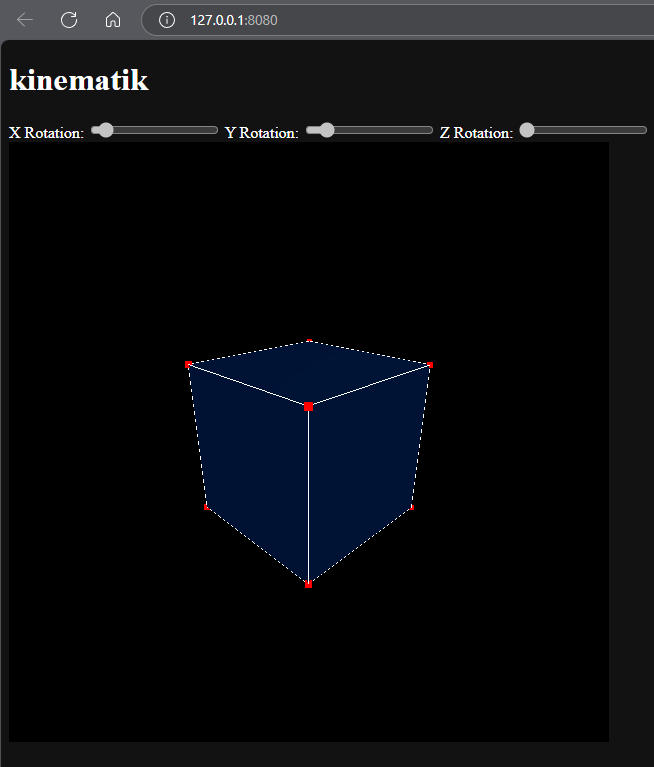
\includegraphics[width=0.7\textwidth]{images/prototyp.PNG}
        \caption{Prototyp mit Three.js}
        \label{fig:Prototyp1}
    \end{figure}

\vspace{1em}
Dabei stellt der schwarze Bereich in Abbildung \ref{fig:Prototyp1} die Szene dar.
Die virtuelle Kamera stellt die Perspektive, aus der die Szene gerendert werden soll, dar und ist daher nicht als Objekt in der Abbildung zu sehen.
Die ambiente Lichtquelle sorgt dafür, dass der Würfel bei der Farbberechnung seine blaue Farbe beibehält und nicht Schwarz gerendert wird und ist ebenfalls
nicht als Objekt in der Szene zu sehen. Ergänzend dazu sind in der index.html-Datei Schieberegler integriert,
mit denen die Rotation des Würfels über eine Benutzeroberfläche interaktiv gesteuert werden kann.
Der würfel wird pro Animationsframe geringfügig um die x- und y-Achse des körpereigenen Koordinatensystems rotiert.
Dies stellt die grundlegenden Funktionen des Prototyps dar: Die interaktive Steuerung sowie Animation eines 3D-Objekts.
Der Prototyp erfüllt damit die zentralen Anforderungen, indem er eine dynamische 3D-Visualisierung bietet,
bei der der Benutzer oder die Benutzerin in Echtzeit Einfluss auf die Darstellung nehmen kann.
Diese erste Version des Prototyps ist ein wichtiger Schritt, um die Funktionalität und Flexibilität von Three.js für das Projekt zu validieren.







Ein offensichtlicher Nachteil dieses Ansatzes ist jedoch, dass die visuelle Darstellung des Würfels in einem separaten Browser-Tab läuft.
Die Python-Schnittstelle, die für das eigentliche Framework vorgesehen ist, würde jedoch in der JupyterLab-Umgebung und somit ebenfalls in einem eigenen Tab ausgeführt werden.
Trotz dieser Einschränkung bestätigt der Prototyp, dass Three.js die benötigten Basisfunktionalitäten bereitstellt.

\subsection{Pythreejs-Prototyp}
Der Nachteil, dass die visuelle Darstellung in einem separaten Browser-Tab erfolgt,
lässt sich umgehen, indem man eine Python-basierte Schnittstelle verwendet, die direkt im JupyterLab-Umfeld arbeitet.
Hierzu bietet sich die Bibliothek Pythreejs an, ein Wrapper für Three.js, der eine Python-API zur Verfügung stellt,
welche im Hintergrund JavaScript-Code generiert und ausführt.

Pythreejs ist eine auf Jupyter Widgets basierende Notebook-Erweiterung,
die es Jupyter ermöglicht, die WebGL-Fähigkeiten moderner Browser zu nutzen, indem sie \textit{Bindings}\footnote{Bindings sind Schnittstellen, die es ermöglichen,
Funktionen oder Klassen aus einer Programmiersprache in einer anderen zu verwenden.} zur JavaScript-Bibliothek Three.js bereitstellt.
Durch die Einbettung in die jupyter-widgets-Infrastruktur lässt sich Pythreejs nahtlos mit anderen interaktiven Werkzeugen innerhalb von Jupyter-Notebooks kombinieren,
was die Entwicklung komplexer, interaktiver Visualisierungen erheblich erleichtert \doublecite{pythreejs_doc}.

Die API von Pythreejs orientiert sich dabei stark an der von Three.js,
sodass vorhandene Dokumentationen und Ressourcen weitgehend übertragbar sind.
Ein wesentlicher Unterschied liegt im sogenannten Render-Loop: Während Three.js typischerweise kontinuierlich \textit{Frames}\footnote{Frame = Einzelnes Bild innerhalb einer Bildsequenz, das z.\,B. bei Animationen oder beim Rendering erzeugt und angezeigt wird.} rendert,
erlaubt Pythreejs sowohl eine gezielte Einzelbilddarstellung per Aufruf als auch interaktive Darstellungen über spezielle Renderer-Klassen.
Diese ermöglichen Funktionen wie OrbitControls (für das Schwenken, Zoomen und Drehen der Kamera) direkt innerhalb des Notebooks,
ohne dass ein separater Browser-Tab erforderlich ist \doublecite{pythreejs_doc_intro}.

Nach weiteren Tests wurde deutlich, dass Pythreejs im Vergleich zu Three.js einige Einschränkungen mit sich bringt.
Eine zentrale Erkenntnis war, dass sich das rotation-Attribut eines \textit{Mesh}\footnote{Engl. Begriff für ein Netz aus Eckpunkten (Vertices), Kanten und Flächen, das zur Darstellung von 3D-Geometrien verwendet wird.}-Objekts in Pythreejs nicht direkt verändern lässt.
Stattdessen kann das quaternion-Attribut genutzt werden, um die Rotation zu steuern. Das macht es notwendig, Hilfsfunktionen zu implementieren,
die Euler-Winkel in Quaternionen umrechnen. Dieser Schritt ist jedoch unproblematisch, da solche Funktionen ohnehin aus didaktischen Gründen Teil des Frameworks sein sollen.


Auf Basis dieser Erkenntnisse wurde ein erweiterter Prototyp mit Pythreejs erstellt,
bei dem die entwickelten Hilfsfunktionen aus der Datei util.py zum Einsatz kommen.
Abbildung \ref{fig:Prototyp2} zeigt den visuellen Output des Renderers innerhalb des Prototyps,
wobei es sich bei dem Prototyp um ein Jupyter-Notebook handelt.
\vspace{1em}

    \begin{figure}[H]
        \centering
        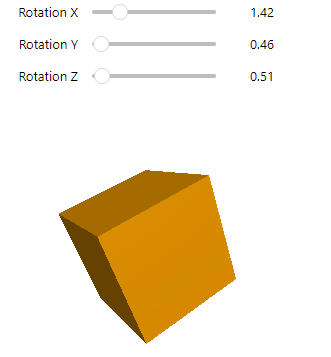
\includegraphics[width=0.7\textwidth]{images/prototyp2.PNG}
        \caption{Notebook-Prototyp mit Pythreejs}
        \label{fig:Prototyp2}
    \end{figure}

\vspace{1em}
Dieser Prototyp zeigte erfolgreich, dass die für das Framework essenziellen Grundfunktionen – insbesondere die Animation und Rotation von Objekten – umsetzbar sind.
Interaktive Elemente konnten hier nicht mehr wie im vorherigen Prototyp durch HTML-Elemente hinzugefügt werden.
Dafür wurde hier die Python-Bibliothek ipywidgets genutzt. 



\subsection{Numpy als Mathematik-Library}
Da der Prototyp verschiedene \textit{numerische}\footnote{Im mathematischen Sinn bedeutet numerisch, dass ein Problem mithilfe von Zahlenwerten und Näherungsverfahren gelöst wird,
anstatt durch exakte symbolische Umformungen.} Berechnungen zur Transformation und Animation von Objekten durchführt,
stellte sich die Frage, welche Bibliothek für die linearen Algebraoperationen am besten geeignet ist.
Obwohl das Framework so gestaltet ist, dass es mit sympy.Matrix-Objekten umgehen kann,
wurde in der konkreten Implementierung bewusst auf NumPy als Rechenbibliothek gesetzt.
Der Grund dafür liegt in der deutlich besseren Effizienz von NumPy bei numerischen Berechnungen.
Während SymPy primär auf \textit{symbolische}\footnote{Im mathematischen Sinn bezeichnet symbolisch die Verarbeitung von Gleichungen und Ausdrücken durch exakte algebraische Umformungen unter Verwendung von Variablen und Symbolen, im Gegensatz zu numerischen Näherungen.} Mathematik ausgelegt ist, wie das Umformen,
Ableiten oder Vereinfachen mathematischer Ausdrücke, ist NumPy auf die schnelle numerische Verarbeitung konkreter Zahlenwerte optimiert.

Das zeigt sich besonders deutlich in der Rechengeschwindigkeit: In einem einfachen Test zur Matrixmultiplikation zweier 100x100-Matrizen benötigte NumPy nur etwa 0.0017
Sekunden. SymPy benötigte für dieselbe Operation rund 9.7 Sekunden, wie man an der folgenden Konsolenausgabe sehen kann:
\begin{center}
    \begin{verbatim}
    NumPy Zeit: 0.001711 Sekunden
    SymPy Zeit: 9.699459 Sekunden
    \end{verbatim}
\end{center}
Der Unterschied liegt dabei nicht im mathematischen Verfahren selbst,
sondern in der Art der Datenverarbeitung: NumPy arbeitet mit kompakten, typisierten Datenstrukturen und nutzt intern optimierte C-Implementierungen,
während SymPy jeden Rechenschritt symbolisch verfolgt und daher deutlich langsamer ist \doublecite{numpy_doc, sympy_doc_advanced_usage}.

Da das Ziel des Frameworks ist, Transformationen numerisch auszuwerten und direkt auf reale Objekte anzuwenden,
war eine symbolische Verarbeitung nicht erforderlich. Dennoch war eine der zentralen Anforderungen, dass das Framework mit sympy.Matrix-Objekten kompatibel ist.
Daher wurde sichergestellt, dass solche Eingaben akzeptiert und automatisch in ein numerisch geeignetes Format überführt werden.
Dadruch bleibt auch bei der Verwendung von SymPy eine korrekte und performante Ausführung gewährleistet. Die Voraussetzung dafür ist jedoch,
dass die über\-gebenen sympy.Ma\-trix-Objekte sich auf konkrete Werte oder Annäherungen zurückführen lassen.

\subsection{Animationslogik}
Darauf aufbauend wurden die Notebooks rotation.ipynb, quader.ipynb und robot.ipynb entwickelt. Parallel dazu wurde die Bibliothek util.py
schrittweise um zusätzliche Funktionen ergänzt, um komplexere Abläufe und Animationen realisieren zu können.
Ein zentrales Prinzip bei der Animationslogik in util.py ist die Verwendung eines zeitbasierten Interpolationsschemas.
Dabei wird die Rotation, Skalierung oder Translation zwischen zwei Zuständen schrittweise überführt.
Der Ablauf folgt dabei einem einfachen Muster:

\begin{algorithm}
    \caption{Interpolation einer Transformation}
    \begin{algorithmic}[1]
    \State $speed$ \Comment{Interpolationsgeschwindigkeit}
    \State $t \gets 0$
    \State $\Delta t \gets 0.002$
    \While{$t \leq 1$}
        \State $mesh.transform \gets \mathit{interpolate}(old\_transform, new\_transform, t)$
        \State $t \gets t + \Delta t$
        \State $\mathit{wait}(1/speed)$
    \EndWhile
    \State $mesh.transform \gets \mathit{interpolate}(old\_transform, new\_transform, 1)$
    \end{algorithmic}
\end{algorithm}

Dabei beschreibt t den Fortschritt der Interpolation von 0 bis 1, delta ist die Schrittweite, welche einen kleinen Wert haben sollte damit die Animation flüssig läuft.
In jedem Schritt wird eine neue Zwischen-Rotation, Position oder Skalierung berechnet und auf das Objekt angewendet, sodass eine flüssige Bewegung entsteht.
Bei der praktischen Umsetzung des Algorithmus wurde die python library time für das Warten verwendet. Es fiel auf,
dass time.sleep() ab einem gewissen Schwellenwert (etwa <1ms) keine weiteren Verkürzungen der Wartezeit bewirkt.
Dies liegt vermutlich an dem overhead der Funktion. Auch wenn kleinere Werte übergeben werden,
wird faktisch immer eine Mindestwartezeit eingehalten, die sich technisch nicht weiter reduzieren lässt.
Dadurch war die Steuerung der Animationsgeschwindigkeit unterhalb dieser Grenze nicht mehr differenzierbar.

\subsection{Environment-Klasse}
Zum Ende der Entwicklungsarbeit hin wurde klar, welche Gemeinsamkeiten die Szenarien in rotation.ipynb, quader.ipynb und robot.ipynb und womöglich auch zukünftige Aufgabentypen haben.
So wurde die Klasse Environment entworfen, die wiederkehrende Elemente in einer flexiblen und erweiterbaren Struktur zusammenfasst.

Die Klasse Environment kapselt die Erstellung und Verwaltung einer dreidimensionalen Szene.
Dabei werden grundlegende Bestandteile wie Kamera, Lichtquellen, Gitter und Achsenobjekte automatisch erzeugt und zu einer Scene-Instanz zusammengefügt.
Darüber hinaus integriert die Klasse ein interaktives Renderer-Element mit Kamera-Steuerung (OrbitControls),
das direkt im Notebook angezeigt wird.

Um eine besonders einfache Erweiterbarkeit zu gewährleisten, wurden Methoden wie add, add\_widget und add\_gizmo\_controls hinzugefügt,
die beliebige Objekte und interaktive Steuerelemente zur Szene hinzufügen.

Die Environment-Klasse übernimmt somit eine zentrale Rolle innerhalb des Frameworks.
Sie abstrahiert technische Details der Visualisierung und erlaubt es, sich auf die inhaltliche Modellierung von Bewegungsabläufen zu konzentrieren.
Dadurch soll die Entwicklung und Darstellung von Aufgaben in den Notebooks rotation.ipynb, quader.ipynb und robot.ipynb vereinfacht werden.

Die Kombination aus pythreejs, den in util.py enthaltenen Transformationsfunktionen und der Environment-Klasse bildet
somit ein Fundament für die weitere Entwicklung des Frameworks.
Erweiterungen wie die Entwicklung aufgabenbezogener Rotationsszenarien oder die schrittweise Analyse
komplexerer Bewegungsabläufe lassen sich auf dieser Basis modular und interaktiv umsetzen.


